\documentclass{zc-ust-hw}

\usepackage{booktabs}
\usepackage{microtype}
\graphicspath{{../plots/phase1/}}
\hypersetup{colorlinks=true, linkcolor=black, citecolor=black, urlcolor=blue!60!black}
\lstset{language=C++, numbers=none, basicstyle=\ttfamily\footnotesize}
\setlist{itemsep=2pt, topsep=4pt}

% Title block: name / ID / date in a wrapping column beside the logo, so long name or ID
% lists continue on the next line instead of running under the logo.
\makeatletter
\renewcommand{\maketitle}{%
  \noindent
  \begin{minipage}[t]{0.76\linewidth}
    \vspace{0pt}
    \begin{tabular}[t]{@{}l p{0.82\linewidth}@{}}
      \ifx\@name\empty\else Name: & \raggedright \@name \tabularnewline \fi
      \ifx\@id\empty\else ID: & \raggedright \@id \tabularnewline \fi
      Date: & \today
    \end{tabular}
  \end{minipage}\hfill
  \begin{minipage}[t]{0.2\linewidth}
    \vspace{0pt}\raggedleft
    
\includegraphics[height=2cm]{logo.jpg}
  \end{minipage}

  \begin{center}
    \textbf{\large \@course}\\
    \@assignment
  \end{center}

  \noindent\rule{\linewidth}{0.1mm}
  \medskip
}
\makeatother

\newcommand{\repo}{\url{https://github.com/AliAshraf69420/Parallel-Distributed-Project}}

\name{Ali Ashraf Hassan Abdelghany, Ahmad Muhammadi, Omar Ali, Abdullah Ayman}
\id{202301812, 202301826, 202300942, 202301731}
\course{SW 401}
\assignment{Phase 1 Report}

\begin{document}

\maketitle

\noindent\textbf{Repository:} \repo\ (reproduction steps in \texttt{README.md}).\\
\textbf{Machine:} AMD Ryzen 7 5800H, 8 cores / 16 threads, L1d 32\,KiB and L2 512\,KiB per core,
L3 16\,MiB shared, 14\,GiB RAM, NVMe SSD, Arch Linux 7.2, GCC 16.2
(\texttt{-O3 -march=native -ffp-contract=off}).

%======================================================================
\section{Dataset and preprocessing}
%======================================================================

We use \textbf{CUB-200-2011} (Caltech-UCSD Birds), approved by the instructor: 11{,}788
JPEG photographs of 200 bird species, with an official train/test split and one bounding box
per image. Decoded to raw RGB, the images are 5.9\,GiB, which is the data every implementation
processes. The project doubles as a data pipeline for a later model-training project, so the
computation is the standard input preparation for an image classifier.

Preprocessing is in Python (\texttt{preprocessing/}, conda environment \texttt{sw401}, which
pins Pillow~11.3 and libjpeg-turbo~3.1 so everyone decodes to identical pixels):
\begin{enumerate}
  \item \textbf{Validate} (\texttt{validate.py}). Every JPEG is fully decoded. Images are dropped
    if metadata is missing, the file is missing or corrupt, the bounding box is degenerate after
    clamping (narrower or shorter than 8\,px), or the decoded pixels duplicate an earlier image
    (SHA-1 of the pixels). Non-RGB images are converted to RGB. Boxes are rounded outward to
    integer pixels and clamped to the image.
  \item \textbf{Predecode} (\texttt{predecode.py}). Each image is decoded \emph{once} into raw HWC
    RGB bytes at its original size, in 1\,GiB shards, with an index of 32-byte records
    (offset, id, class, split, size, box). Blocks are 64-byte aligned. The set is verified by
    re-hashing every block before it is moved into place.
  \item \textbf{Subsets} (\texttt{make\_subsets.py}). Class- and split-stratified, nested
    subsets by decoded size: 100\,MB and 500\,MB for the experiments, and $p\times700$\,MiB
    ($p=1,2,4,8$) for weak scaling.
  \item \textbf{Reference} (\texttt{reference.py}). A NumPy implementation of the computation
    produces the frozen expected output (Section~\ref{sec:problem}).
\end{enumerate}

\begin{table}[H]
\centering\small
\begin{tabular}{lrr}
\toprule
 & Before & After \\
\midrule
Images (train / test) & 11{,}788 (5{,}994 / 5{,}794) & 11{,}787 (5{,}993 / 5{,}794) \\
Classes & 200 & 200 \\
Size & 1.07\,GiB JPEG & 5.90\,GiB raw RGB (6 shards) \\
\midrule
Dropped & \multicolumn{2}{l}{1 duplicate (id 3340 is byte-identical to id 3310, same class, both train);} \\
 & \multicolumn{2}{l}{0 corrupt, 0 missing, 0 degenerate boxes} \\
Converted / clamped & \multicolumn{2}{l}{8 grayscale images converted to RGB; 30 boxes clamped to the image} \\
\midrule
Subsets & \multicolumn{2}{l}{100MB: 195 images (147 classes); 500MB: 971 images (200 classes)} \\
\bottomrule
\end{tabular}
\caption{Dataset before and after preprocessing (\texttt{results/preprocessing/}).
Validation takes 4\,s and predecoding 22\,s with 16 processes.}
\end{table}

%======================================================================
\section{Problem statement and baseline design}\label{sec:problem}
%======================================================================

For every image, the pipeline produces the tensor a classifier is trained on:
\begin{enumerate}
  \item \textbf{Crop and resize:} crop to the bounding box and resize to $224\times224$
    with bilinear interpolation.
  \item \textbf{Pass 1, channel statistics:} the mean $\mu_c$ and standard deviation $\sigma_c$
    of each colour channel over all \emph{training} images. This is a global reduction over
    $3.0\times10^8$ values per channel.
  \item \textbf{Pass 2, normalize:} $x' = (x/255-\mu_c)/\sigma_c$ for every image, written as
    a channel-first float32 tensor (588\,KiB per image).
\end{enumerate}
Normalizing per channel centres the inputs and gives every channel unit variance, which keeps
gradients well conditioned. The statistics come from the training split only (no test leakage)
and are the same for every image, because the class is unknown at inference time. On the full
set we obtain $\mu = (0.4718, 0.4709, 0.4057)$ and $\sigma = (0.2356, 0.2317, 0.2583)$,
close to the usual ImageNet values.

\paragraph{Exact by construction.} So that every implementation (sequential, OpenMP, threads,
and later MPI and Hadoop) can be checked \emph{bit for bit} instead of within a tolerance, the
computation is specified with integers: a fixed-point bilinear resize with 11-bit weights,
exact integer sums $n$, $\sum v$, $\sum v^2$ per channel (merging partial results is integer
addition, so the result is independent of thread count and order), and a 256-entry float32
lookup table per channel computed in IEEE double. FMA contraction is disabled
(\texttt{-ffp-contract=off}). The fixed-point resize stays within 0.56 grey levels of a float
bilinear resize.

\paragraph{Baseline.} \texttt{src/common/} holds the set reader (shards are \texttt{mmap}ed), the
kernels and the per-image work of each pass. \texttt{src/seq/main.cpp} is two loops: pass 1 over
the training images (resize, accumulate), then pass 2 over all images (resize again, normalize,
and a CRC-32 of the resized and of the normalized image). Each run writes its statistics and
per-image CRCs, and \texttt{tests/check.py} compares them with the reference. Every run in this
report passed. On the full set the sequential baseline takes \textbf{9.79\,s} of compute
(pass 1: 2.07\,s, pass 2: 7.59\,s) and 10.06\,s end to end.

%======================================================================
\section{Parallelization approach}
%======================================================================

\paragraph{OpenMP} (\texttt{src/omp/main.cpp}). Each image is independent, so both passes are a
\texttt{parallel for} over images, with \texttt{schedule(runtime)} so the schedule can be chosen
on the command line. Pass 1 needs a reduction over a struct of seven 64-bit counters, which is a
user-defined reduction. Every thread accumulates privately, and there is no \texttt{critical} or
\texttt{atomic} in the loop:
\begin{lstlisting}
#pragma omp declare reduction(merge : cub::Stats : omp_out.merge(omp_in)) \
        initializer(omp_priv = cub::Stats{})
#pragma omp parallel
{
    std::vector<uint8_t> scratch(kResizedBytes);    // one buffer per thread
    #pragma omp for schedule(runtime) reduction(merge : st)
    for (long k = 0; k < n_train; ++k)
        pass1_record(ds, train[k], scratch.data(), st);
}
\end{lstlisting}
Pass 2 writes only per-image slots (two CRCs, and optionally its own block of the output file
via \texttt{pwrite}), so it needs no synchronization. The implicit barrier between the two
parallel regions is the only synchronization point. Threads are pinned one per physical core
(\texttt{OMP\_PROC\_BIND=close}, \texttt{OMP\_PLACES=cores}).

{\sloppy
\paragraph{C++ threads} (\texttt{src/threads/main.cpp}). A producer--consumer pipeline built
from \texttt{std::thread}, \texttt{std::mutex}, \texttt{std::}\allowbreak\texttt{condition\_variable} and
\texttt{std::atomic}: a reader thread prefetches each image (\texttt{madvise}) and pushes its
index into a bounded queue; $N$ pinned workers pop and process images; with \texttt{--write}, a
writer thread receives finished tensors through a second bounded queue and recycles buffers.
Pass-1 partial statistics are \texttt{alignas(64)} per worker and merged after
\texttt{join()}.\par}

%======================================================================
\section{Performance results}
%======================================================================

\paragraph{Method.} Every configuration gets one discarded warm-up run and three measured runs,
and we report the median. The data is preloaded into the page cache, so the times measure
compute, not disk. ``Compute'' is pass 1 + merge + pass 2; ``total'' also includes opening the
set and writing the result files (\texttt{scripts/bench/phase1.py}, raw rows in
\texttt{results/timings/}).

\begin{table}[H]
\centering\small
\begin{tabular}{rrrrrrrrr}
\toprule
$p$ & pass 1 (s) & pass 2 (s) & compute (s) & $S$ & $E$ & $f$ & total (s) & $S_\text{total}$ \\
\midrule
1 & 2.070 & 7.585 & 9.675 & 1.01 & 1.01 & -- & 9.929 & 1.01 \\
2 & 1.055 & 3.958 & 5.013 & 1.95 & 0.98 & 0.024 & 5.272 & 1.91 \\
4 & 0.559 & 2.082 & 2.635 & 3.72 & 0.93 & 0.025 & 2.891 & 3.48 \\
8 & 0.294 & 1.059 & 1.355 & \textbf{7.23} & 0.90 & 0.015 & 1.604 & 6.27 \\
16 (SMT) & 0.272 & 0.865 & 1.123 & 8.72 & 0.55 & 0.056 & 1.385 & 7.26 \\
\bottomrule
\end{tabular}
\caption{OpenMP strong scaling on the full set (static schedule). $S=T_S/T_p$ with
$T_S=9.79$\,s, $E=S/p$, $f=(1/S-1/p)/(1-1/p)$. The C++ threads pipeline is within 3\,\%
(7.30$\times$ at $p=8$). At $p=8$ the 100MB and 500MB sets reach 6.79$\times$ and
6.43$\times$.}
\label{tab:strong}
\end{table}

\begin{figure}[H]
\centering
\begin{subfigure}{0.49\linewidth}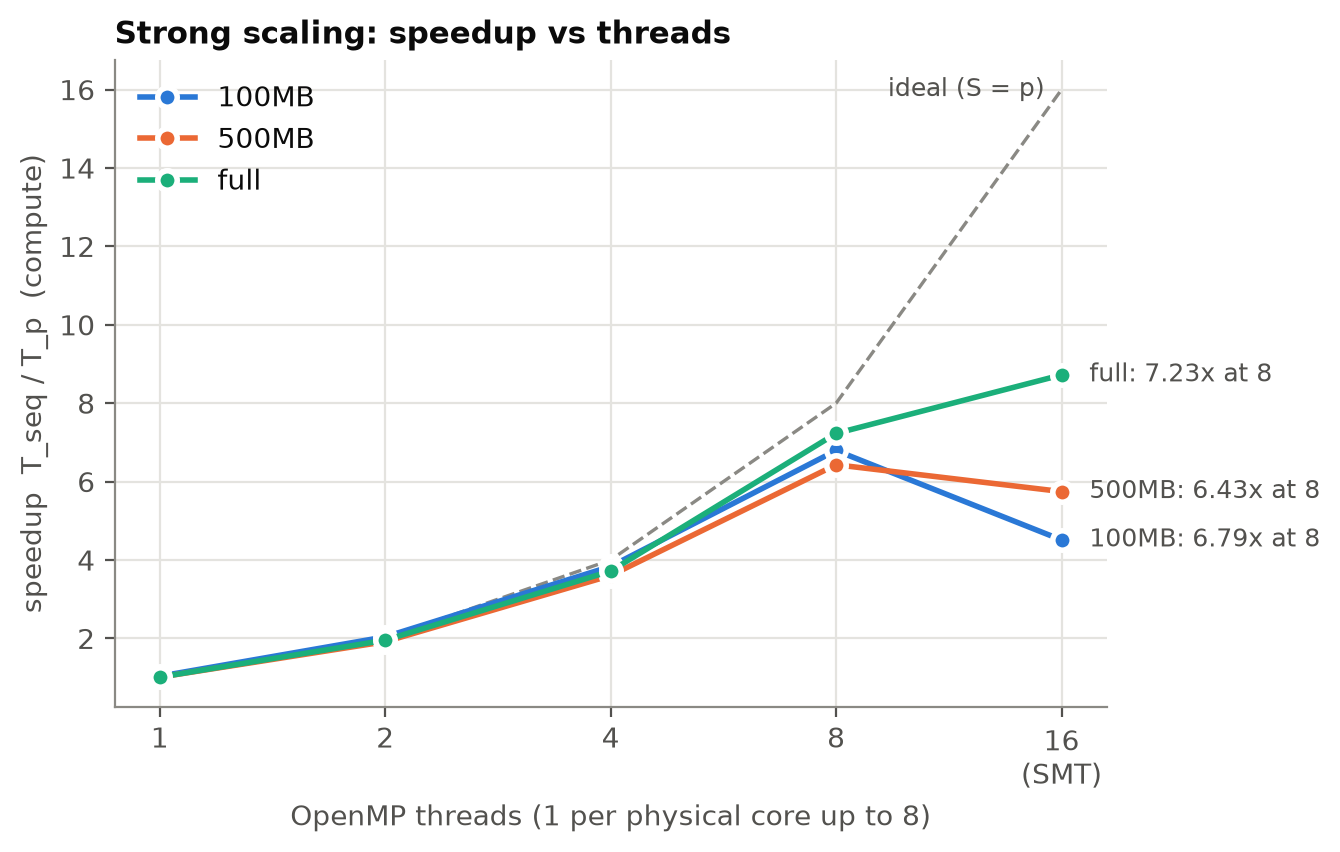
\includegraphics[width=\linewidth]{speedup.png}\end{subfigure}\hfill
\begin{subfigure}{0.49\linewidth}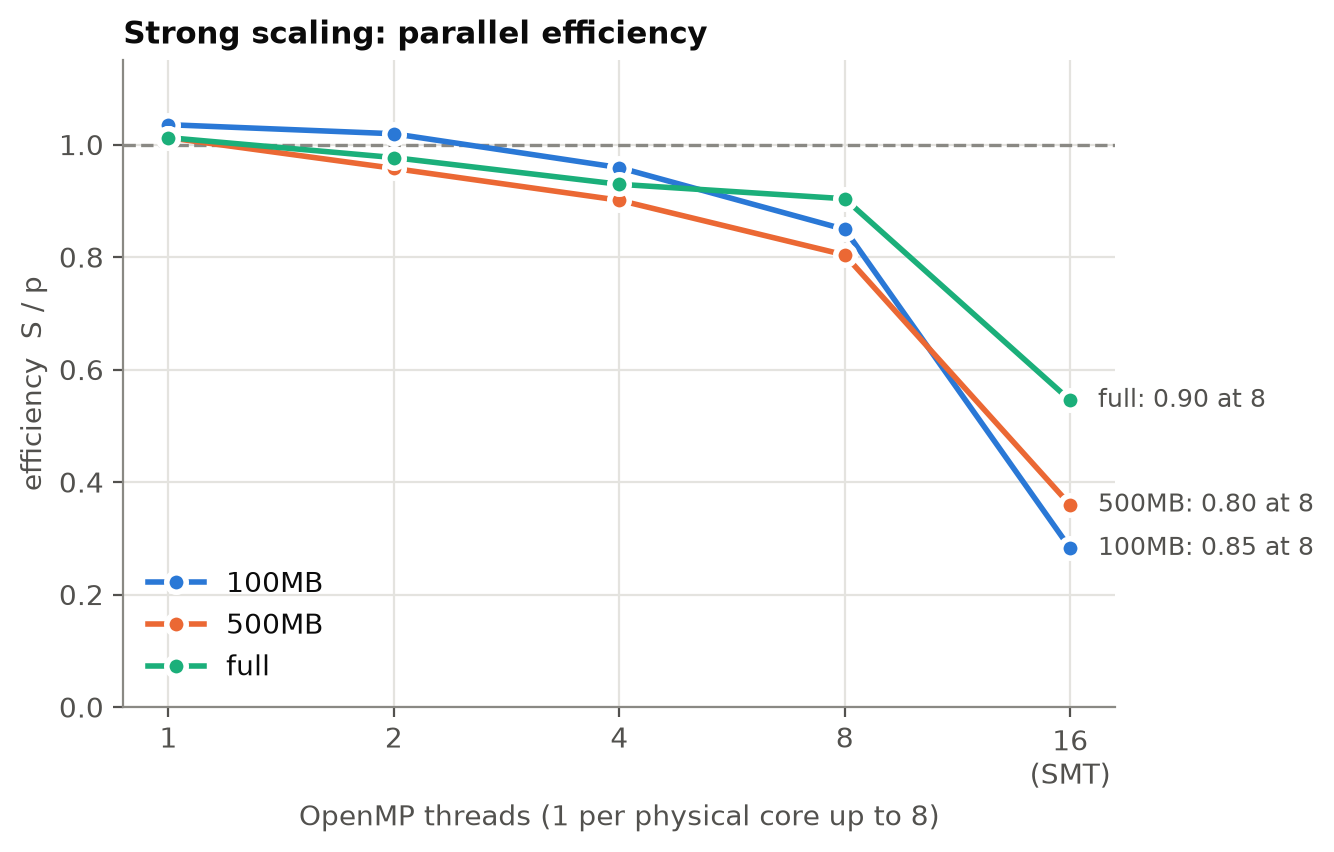
\includegraphics[width=\linewidth]{efficiency.png}\end{subfigure}
\caption{Speedup and efficiency against threads, per dataset (compute time).}
\label{fig:strong}
\end{figure}

Scaling is close to linear up to the 8 physical cores. The full set reaches $7.23\times$
($E=0.90$). The smaller sets scale slightly worse, because fixed costs (thread start-up, the
barrier between the passes) are a larger share of a 25\,ms run, and because the 100MB set has
only 24 images per thread, so a one-image imbalance is 4\,\%. With 16 threads, SMT adds a
further 21\,\% on the full set. On the small sets, OpenMP gets \emph{slower} at 16 threads
(100MB: 4.5$\times$), while the threads pipeline still reaches 8.2$\times$. Our explanation is
that OpenMP threads spin-wait at barriers and steal cycles from their working SMT sibling,
whereas idle pipeline workers sleep on a condition variable.

\paragraph{Scheduling.} We compared \texttt{static}, \texttt{static,1}, \texttt{dynamic,1},
\texttt{dynamic,16} and \texttt{guided} at 4 and 8 threads, in storage order and with the
largest crops first (\texttt{--order area-desc}, the worst case for block-static scheduling).
\textbf{All schedules are within 4\,\% of each other} (full set, 8 threads: 1.60--1.67\,s,
Figure~\ref{fig:sched}). We had expected dynamic scheduling to win, because crop areas vary 24
times. Measuring the per-image time shows why it does not (Figure~\ref{fig:records}): the resize
cost depends on the fixed $224\times224$ \emph{output}, not on the crop size, so the work per
image is almost uniform (coefficient of variation 0.03, 95th/5th percentile ratio 1.10,
correlation with crop area 0.01). With uniform work, \texttt{static} is the best choice (no
scheduling overhead, contiguous blocks). The one clear loser is \texttt{dynamic,16} on the 100MB
set: 195 images make only 13 chunks for 8 threads, so some threads get two chunks and the rest
one.

\begin{figure}[H]
\centering
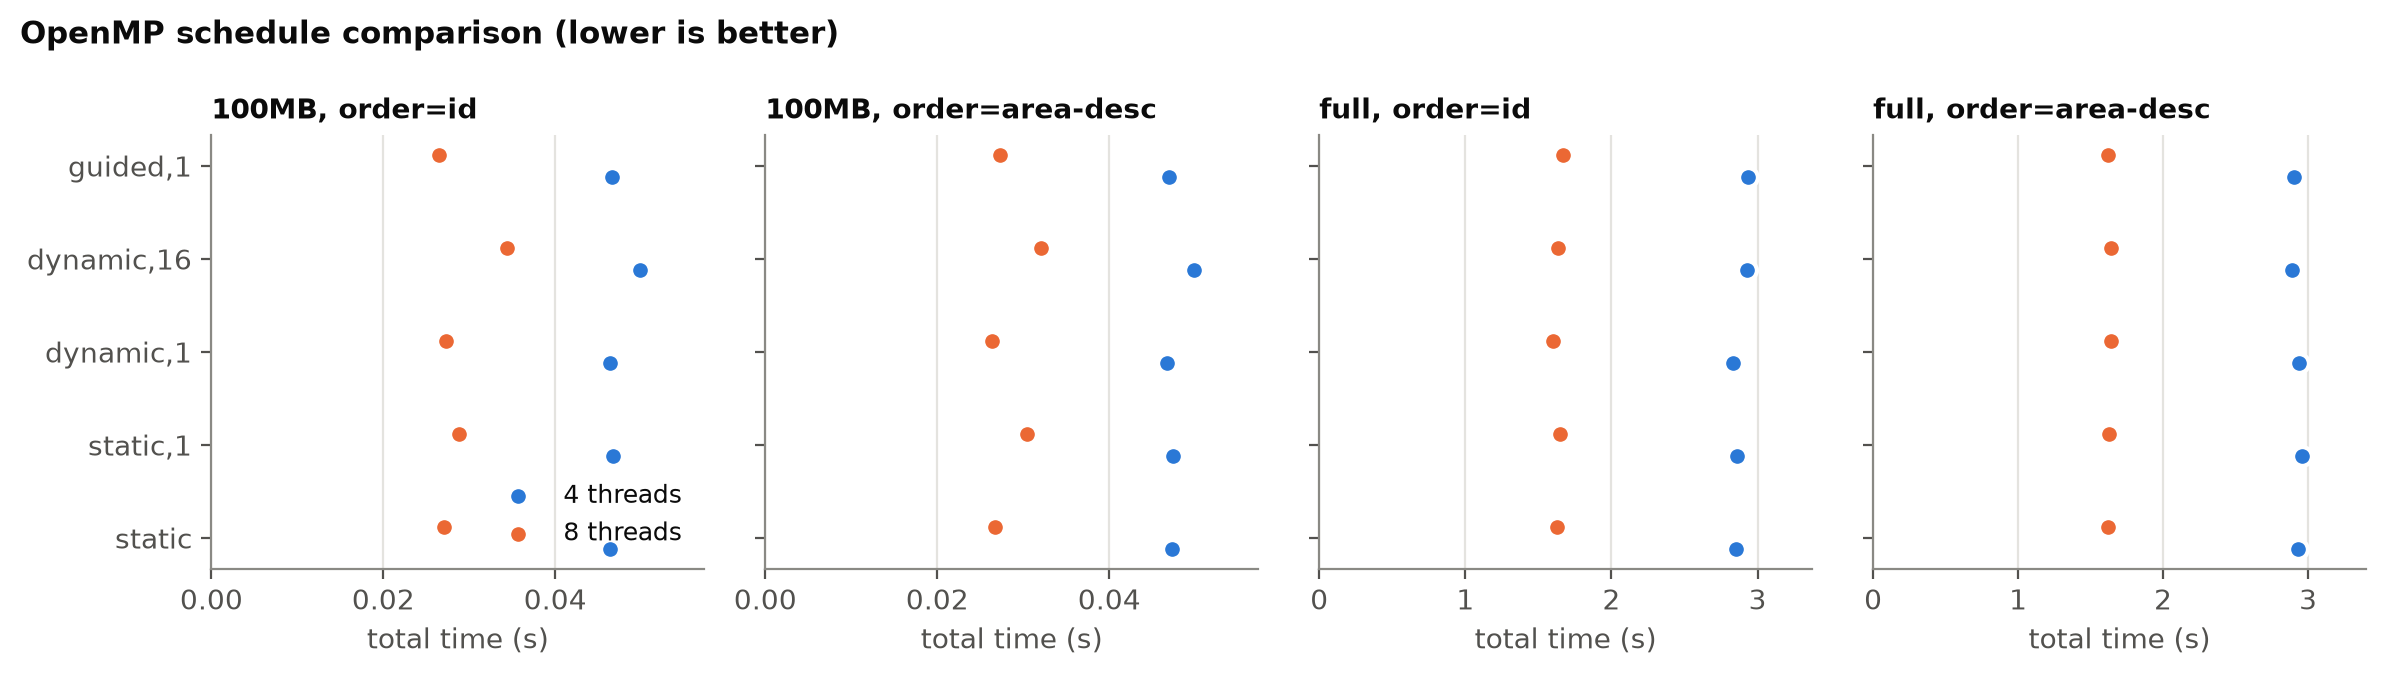
\includegraphics[width=\linewidth]{schedule.png}
\caption{Total time per schedule (median of 3), 4 and 8 threads.}
\label{fig:sched}
\end{figure}

%======================================================================
\section{Amdahl, Gustafson, and profiling}
%======================================================================

\paragraph{Amdahl.} The experimentally determined serial fraction of the compute is small and
stable ($f\approx0.015$--$0.025$, Table~\ref{tab:strong}). That bounds the compute speedup at
$1/f\approx40$--$66$, far above 8 cores. Predicting $p=8$ from the $p=2$ value
($f=0.024$) gives $S=6.9$, against 7.23 measured. End to end, opening the set (index read and
page-cache check, about 0.25\,s) is serial and raises $f$ to 0.039, which caps the end-to-end
speedup at about 25. The merge of the statistics takes 1\,\textmu s and is negligible.

\emph{What the remaining 10\,\% loss is, then.} \texttt{perf stat} on the full run shows the
same 91.3 billion instructions at 1 and 8 threads, so there is no extra work. The effective
clock falls from 3.93\,GHz with one active core to 3.55\,GHz with eight (all-core boost on a
laptop), and IPC from 2.28 to 2.20. The ratio $3.55/3.93=0.90$ matches the measured efficiency,
so the shortfall is the processor's frequency scaling, not serial code. (The effective clock is
estimated as user-mode cycles divided by CPU time.)

\begin{figure}[H]
\centering
\begin{subfigure}{0.49\linewidth}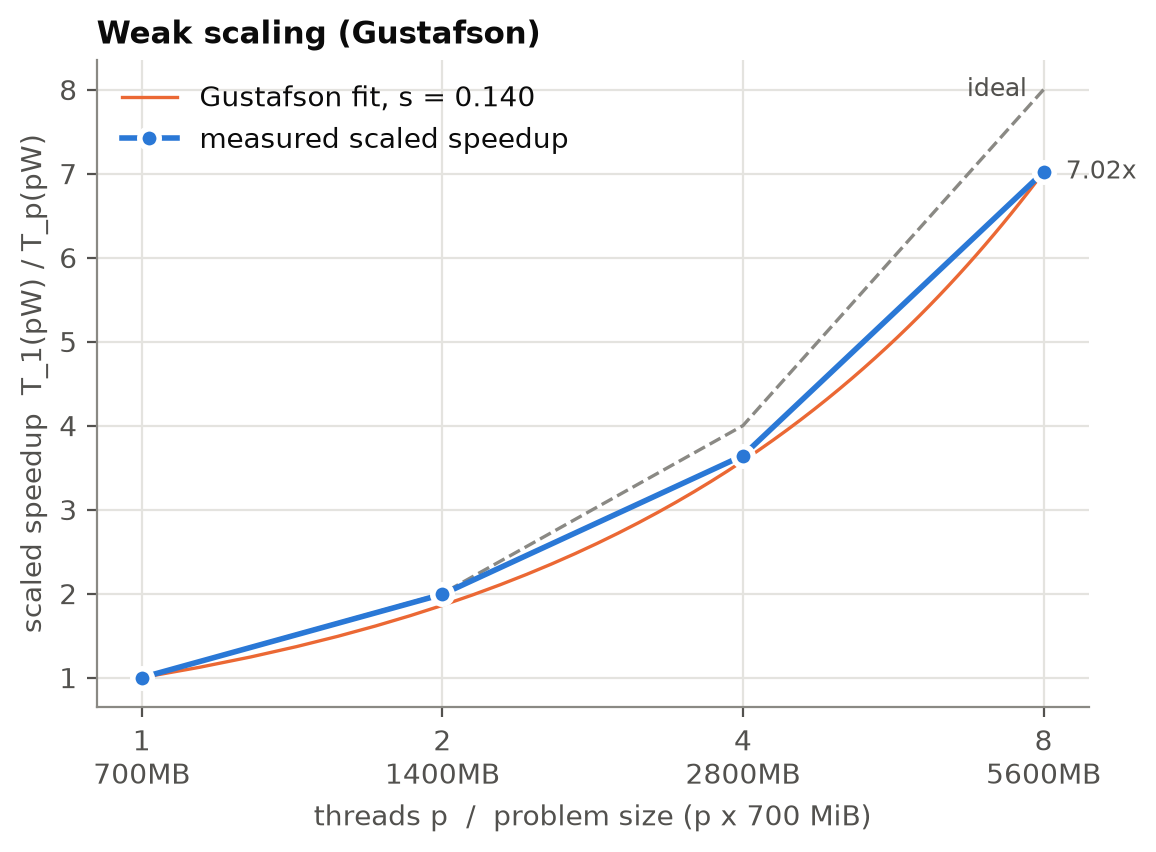
\includegraphics[width=\linewidth]{weak.png}\caption{}\label{fig:weak}\end{subfigure}\hfill
\begin{subfigure}{0.49\linewidth}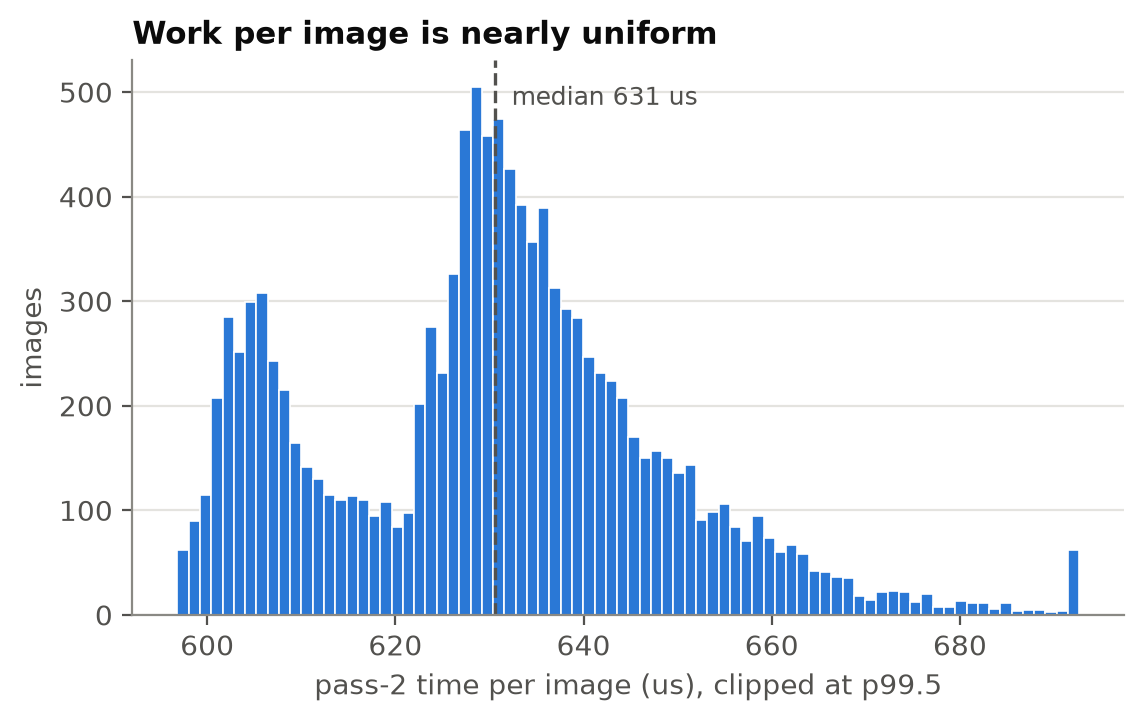
\includegraphics[width=\linewidth]{records.png}\caption{}\label{fig:records}\end{subfigure}
\caption{(a) Weak scaling: $p$ threads on $p\times700$\,MiB. (b) Per-image pass-2 time,
sequential, full set; the last bar collects the slowest 0.5\,\% (axis clipped at p99.5).}
\end{figure}

\paragraph{Gustafson.} Giving each thread 700\,MiB, the compute time grows only from 1.10\,s
($p=1$) to 1.27\,s ($p=8$). The scaled speedup is \textbf{7.02} at $p=8$ (weak efficiency 0.87,
Figure~\ref{fig:weak}). Fitting $S(p)=p-s(p-1)$ gives $s=0.14$. This $s$ is not serial code:
it is the slower clock and the shared L3 and memory bandwidth seen above. As Gustafson
predicts, a larger problem keeps all cores busy, and the full set scales better than the 100MB
set.

\paragraph{Memory hierarchy} (\texttt{src/memexp/}). A pointer chase through random 64-byte
lines (Figure~\ref{fig:mem}a) shows load latencies of 1.2\,ns (L1, $\le$32\,KiB),
3.1--3.6\,ns (L2, $\le$512\,KiB), 9--13\,ns (L3, $\le$8\,MiB) and 65--122\,ns (DRAM), with the
steps exactly at the cache sizes. A stride sweep over 1\,GiB of our shard bytes
(Figure~\ref{fig:mem}b) shows the cost per access rising until every access touches a new
64-byte line, and again at 4\,KiB, where the hardware prefetcher stops at page boundaries. For
our data: a typical crop (about 166\,KB) and the resized image (147\,KiB) fit in L2, but the
588\,KiB float tensor does not, so normalization and its CRC stream through L3. This is part
of why pass 2 is 78\,\% of the run time.

\begin{figure}[H]
\centering
\begin{subfigure}{0.49\linewidth}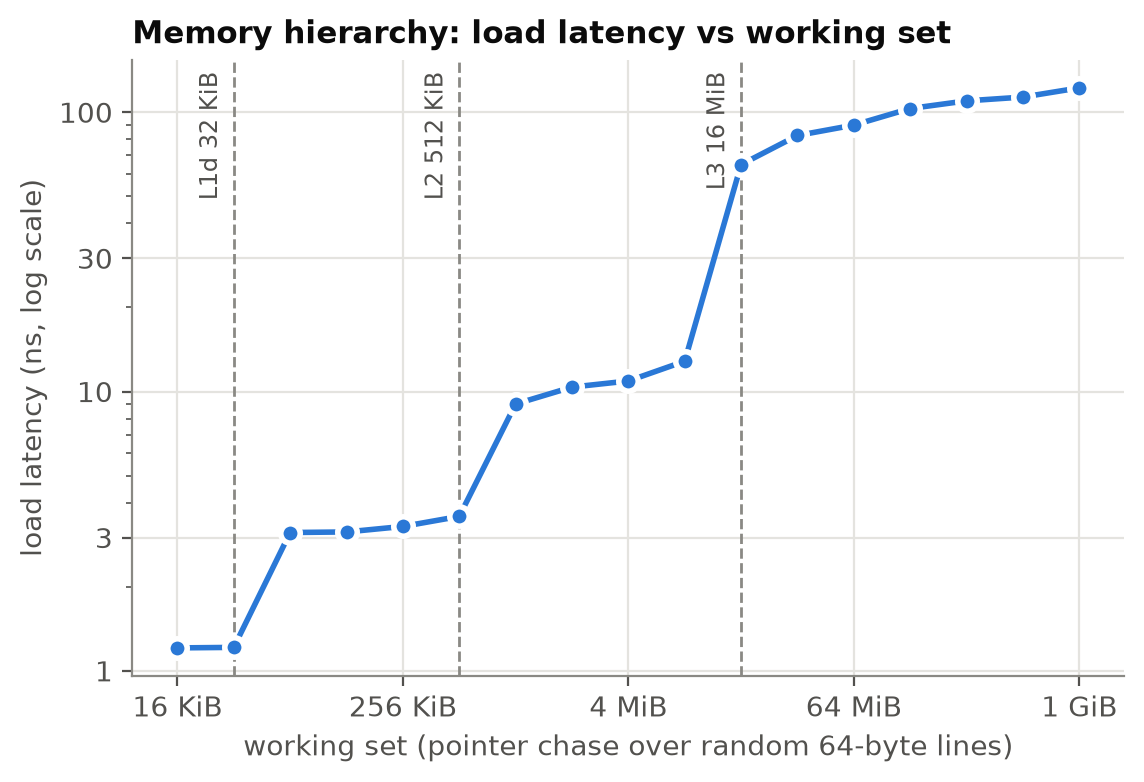
\includegraphics[width=\linewidth]{latency.png}\caption{}\end{subfigure}\hfill
\begin{subfigure}{0.49\linewidth}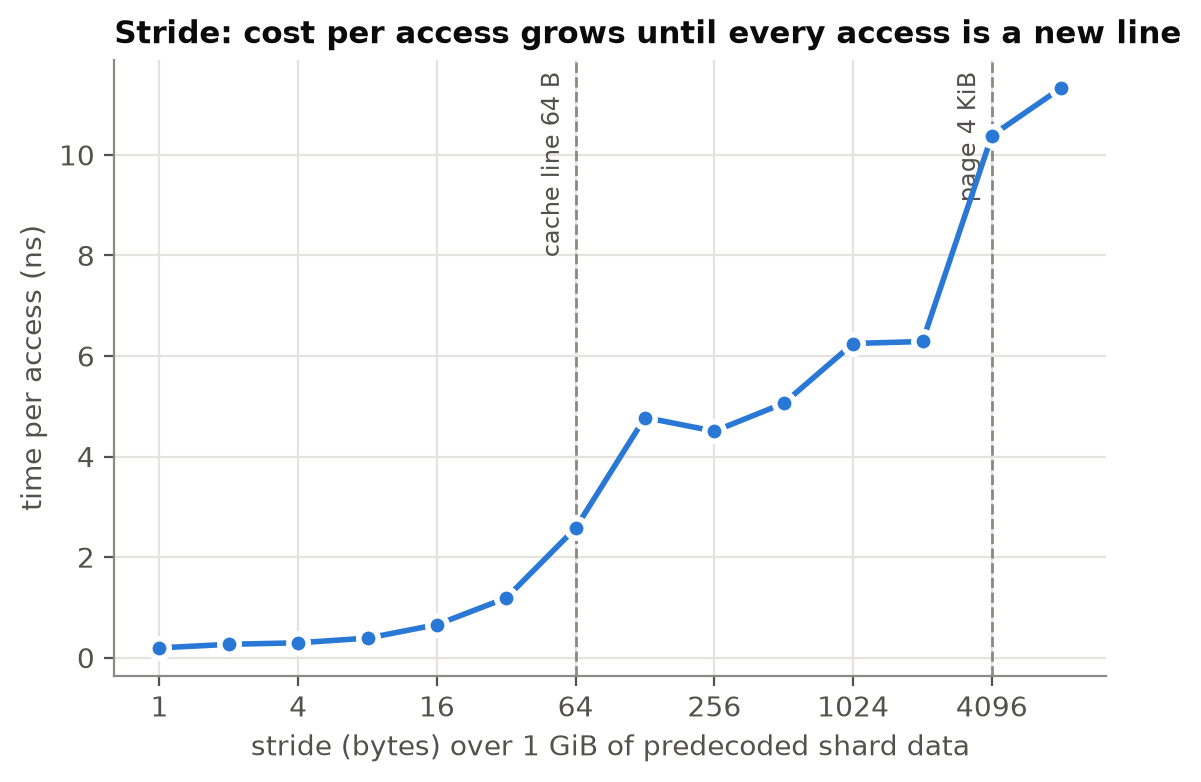
\includegraphics[width=\linewidth]{stride.png}\caption{}\end{subfigure}
\caption{(a) Load latency against working-set size. (b) Time per access against stride.}
\label{fig:mem}
\end{figure}

\paragraph{Locality of our own layout.} We ran the real resize in its row-major traversal and in
a column-major traversal (identical output, verified by CRC) under \texttt{perf stat} (500MB
set, one thread, Table~\ref{tab:perf}). Column-major causes 27 times more cache misses and 5
times more L1 misses, but is only 12\,\% slower. Consecutive output pixels in a column read
different source rows, so almost every access touches a new cache line. But one column touches
only $2\times224$ lines (28\,KiB), these are reused by the next $\approx$21 columns (a line
holds 21 pixels) and stay in L2, so the misses cost L2 latency, and out-of-order execution
overlaps much of it.

\paragraph{False sharing.} Eight threads updating a per-thread pixel-sum counter in memory for
every pixel, with the counters \emph{packed} into one array (three threads per cache line), run
\textbf{17.9 times} slower than accumulating in registers. They also show 3.5 times the cache
misses and 2.3 billion extra cycles, because the line ping-pongs between cores. Padding each
counter to its own 64-byte line removes almost all of it (1.2 times). Our implementations
accumulate in registers per image and merge once per image (OpenMP reduction, padded per-worker
\texttt{Stats} in the pipeline), so they have no shared counters in the hot loop.

\begin{table}[H]
\centering\small
\begin{tabular}{lrrrrr}
\toprule
Variant & Time & Cycles & Cache refs & Cache misses & L1d misses \\
\midrule
Resize, row-major & 377\,\textmu s/img & 1511\,M & 18.2\,M & 2.4\,M & 4.9\,M \\
Resize, column-major & 423\,\textmu s/img & 1757\,M & 134.9\,M & 64.0\,M & 26.2\,M \\
\midrule
Counters packed (8 thr.) & 100.2\,ms & 5738\,M & -- & 19.7\,M & 21.8\,M \\
Counters padded (8 thr.) & 6.7\,ms & 3444\,M & -- & 5.7\,M & 7.9\,M \\
Counters local (8 thr.) & 5.6\,ms & 3409\,M & -- & 5.7\,M & 8.0\,M \\
\bottomrule
\end{tabular}
\caption{\texttt{perf stat} counters (user mode, whole process, including the shared setup).}
\label{tab:perf}
\end{table}

%======================================================================
\section{Reflection: remaining bottlenecks}
%======================================================================

\begin{itemize}
  \item \textbf{Clock frequency, not code}, accounts for the remaining 10\,\% at 8 threads. On
    this laptop that cannot be removed. It means speedups measured here are a lower bound
    for machines with flat all-core clocks.
  \item \textbf{Pass 2 dominates} (78\,\%). It resizes every image a second time and streams a
    588\,KiB tensor plus two CRCs through L3. Keeping the resized images from pass 1
    (\texttt{--cache}, 1.8\,GB) trades memory for the second resize. Fusing normalization
    with the CRC in one pass over the tensor would cut its L3 traffic.
  \item \textbf{Serial start-up} (about 0.25\,s to open the set) limits the end-to-end speedup
    to 6.27 at 8 threads. In Phase 2 every MPI rank opens only its own part of the data, so
    this cost is also divided.
  \item \textbf{Memory capacity.} The full set (5.9\,GiB) roughly fills the free RAM, so cold
    runs are bound by disk reads. Distributing the data across nodes (Phase 2) removes this.
  \item \textbf{Small inputs} are dominated by fixed parallel overhead (100MB: 25\,ms at
    8 threads), which will matter even more for MPI and Hadoop start-up costs.
\end{itemize}

\end{document}
